\documentclass{article}

\usepackage{graphicx}
\usepackage{tikz}
\usepackage{tikzsymbols}
\usetikzlibrary{calc,patterns,shapes.geometric}
\pagestyle{empty}
\usepackage[margin=0pt]{geometry}
\geometry{papersize={14in,12in}}

\def\centerarc[#1](#2)(#3:#4:#5){\draw[#1] ($(#2)+({#5*cos(#3)},{#5*sin(#3)})$) arc (#3:#4:#5);}

\begin{document}
	\begin{figure}
		\centering
		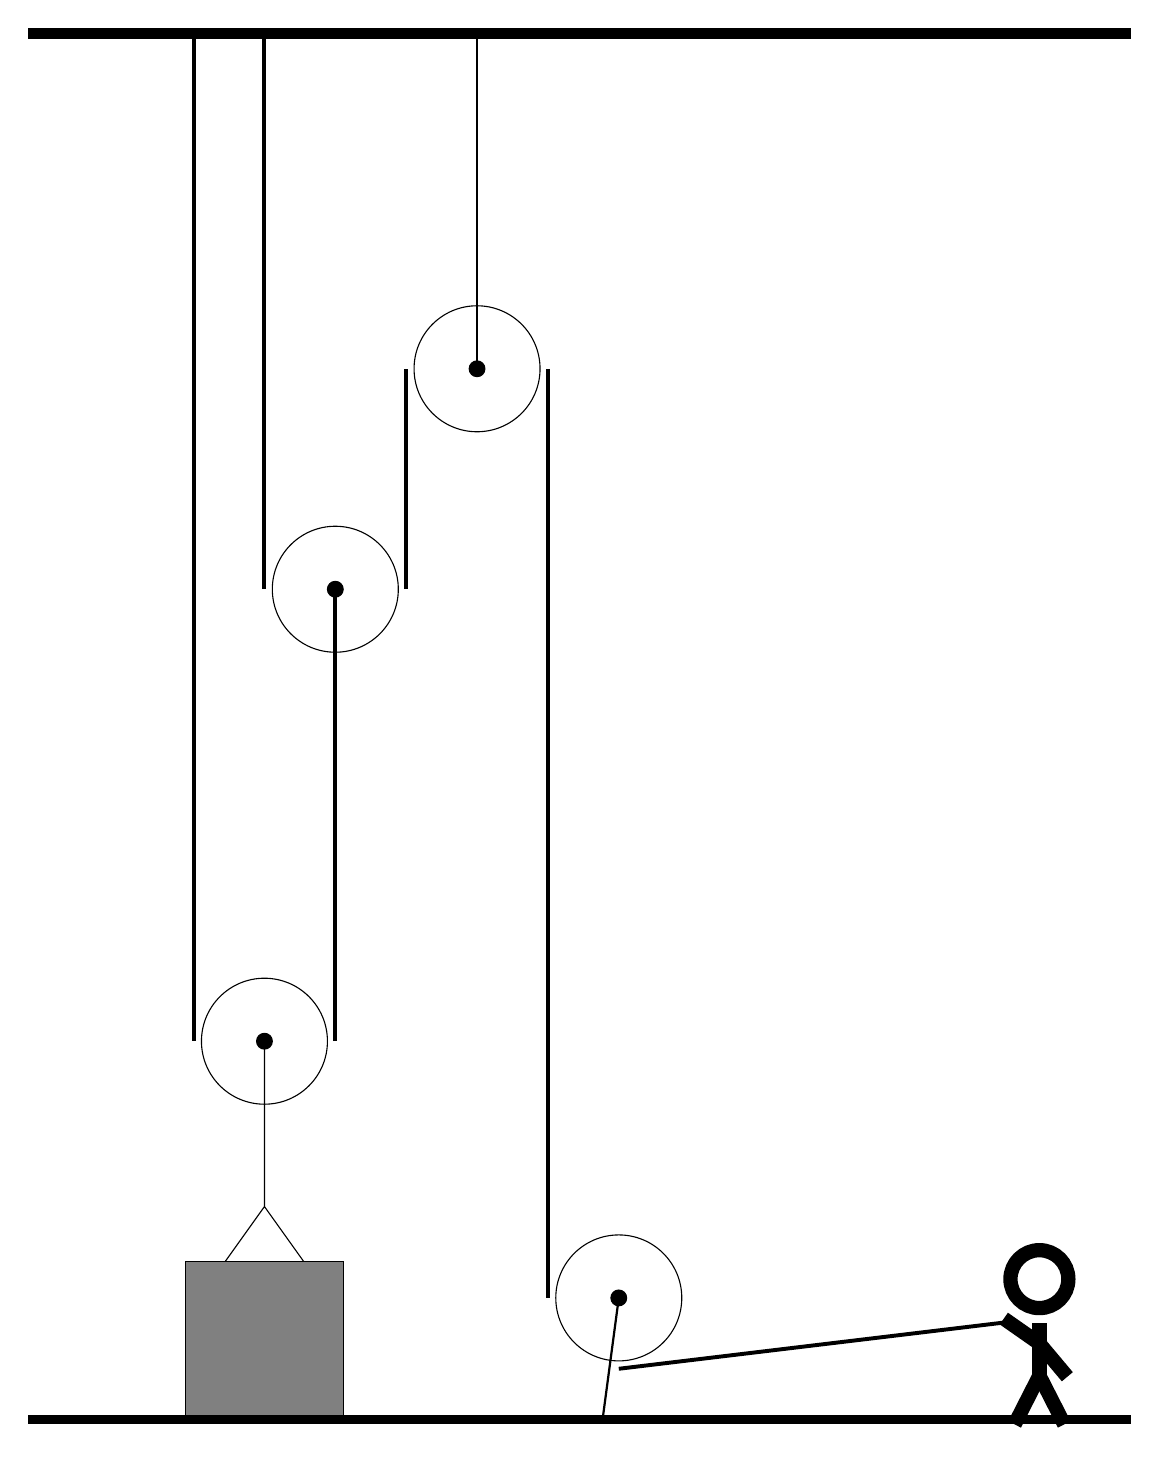
\begin{tikzpicture}
			%%%%% START %%%%%
			\draw[fill=black] (-2, 14) rectangle (12, 14.125);
			
			\draw (1, 1.26) circle (0.8);
			\draw[fill=black] (1, 1.26) circle (0.1);
			
			\draw (1.9, 7.0) circle (0.8);
			\draw[fill=black] (1.9, 7.0) circle (0.1);
			
			\draw (3.7, 9.8) circle (0.8);
			\draw[fill=black] (3.7, 9.8) circle (0.1);
			\draw[thick] (3.7, 9.8) -- (3.7, 14);
			
			\draw (5.5, -2) circle (0.8);
			\draw[fill=black] (5.5, -2) circle (0.1);
			\draw[thick] (5.5, -2) -- (5.3, -3.5);
			
			\draw (1, 1.26) -- (1, -0.84) -- (0.5, -1.54) -- (1.5, -1.54) -- (1, -0.84);
			\draw[fill=black!50] (0, -1.54) rectangle (2, -3.54);
			\draw[line width=0.5mm] (0.1, 14) -- (0.1, 1.26);
			\centerarc[line width=0.5mm](1, 1.26)(180:360:0.9);
			\draw[line width=0.5mm](1.9, 1.26) -- (1.9, 7.0);
			\draw[line width=0.5mm] (1.0, 14) -- (1.0, 7.0);
			\centerarc[line width=0.5mm](1.9, 7.0)(180:360:0.9);
			\draw[line width=0.5mm](2.8, 7.0) -- (2.8, 9.8);
			\centerarc[line width=0.5mm](3.7, 9.8)(0:180:0.9);
			\draw[line width=0.5mm] (4.6, 9.8) -- (4.6, -2);
			\centerarc[line width=0.5mm](5.5, -2)(0:90:-0.9);
			\draw[line width=0.5mm](5.5, -2.9) -- (10.5, -2.3);
			
			\node at (10.8, -2.5) {\Strichmaxerl[10][-35][-50]};
			
			\draw[fill=black] (-2, -3.5) rectangle (12, -3.6);
			%%%%% END %%%%%
		\end{tikzpicture}
	\end{figure}	
\end{document}